% GNUPLOT: LaTeX picture with Postscript
\begingroup
  \makeatletter
  \providecommand\color[2][]{%
    \GenericError{(gnuplot) \space\space\space\@spaces}{%
      Package color not loaded in conjunction with
      terminal option `colourtext'%
    }{See the gnuplot documentation for explanation.%
    }{Either use 'blacktext' in gnuplot or load the package
      color.sty in LaTeX.}%
    \renewcommand\color[2][]{}%
  }%
  \providecommand\includegraphics[2][]{%
    \GenericError{(gnuplot) \space\space\space\@spaces}{%
      Package graphicx or graphics not loaded%
    }{See the gnuplot documentation for explanation.%
    }{The gnuplot epslatex terminal needs graphicx.sty or graphics.sty.}%
    \renewcommand\includegraphics[2][]{}%
  }%
  \providecommand\rotatebox[2]{#2}%
  \@ifundefined{ifGPcolor}{%
    \newif\ifGPcolor
    \GPcolortrue
  }{}%
  \@ifundefined{ifGPblacktext}{%
    \newif\ifGPblacktext
    \GPblacktexttrue
  }{}%
  % define a \g@addto@macro without @ in the name:
  \let\gplgaddtomacro\g@addto@macro
  % define empty templates for all commands taking text:
  \gdef\gplbacktext{}%
  \gdef\gplfronttext{}%
  \makeatother
  \ifGPblacktext
    % no textcolor at all
    \def\colorrgb#1{}%
    \def\colorgray#1{}%
  \else
    % gray or color?
    \ifGPcolor
      \def\colorrgb#1{\color[rgb]{#1}}%
      \def\colorgray#1{\color[gray]{#1}}%
      \expandafter\def\csname LTw\endcsname{\color{white}}%
      \expandafter\def\csname LTb\endcsname{\color{black}}%
      \expandafter\def\csname LTa\endcsname{\color{black}}%
      \expandafter\def\csname LT0\endcsname{\color[rgb]{1,0,0}}%
      \expandafter\def\csname LT1\endcsname{\color[rgb]{0,1,0}}%
      \expandafter\def\csname LT2\endcsname{\color[rgb]{0,0,1}}%
      \expandafter\def\csname LT3\endcsname{\color[rgb]{1,0,1}}%
      \expandafter\def\csname LT4\endcsname{\color[rgb]{0,1,1}}%
      \expandafter\def\csname LT5\endcsname{\color[rgb]{1,1,0}}%
      \expandafter\def\csname LT6\endcsname{\color[rgb]{0,0,0}}%
      \expandafter\def\csname LT7\endcsname{\color[rgb]{1,0.3,0}}%
      \expandafter\def\csname LT8\endcsname{\color[rgb]{0.5,0.5,0.5}}%
    \else
      % gray
      \def\colorrgb#1{\color{black}}%
      \def\colorgray#1{\color[gray]{#1}}%
      \expandafter\def\csname LTw\endcsname{\color{white}}%
      \expandafter\def\csname LTb\endcsname{\color{black}}%
      \expandafter\def\csname LTa\endcsname{\color{black}}%
      \expandafter\def\csname LT0\endcsname{\color{black}}%
      \expandafter\def\csname LT1\endcsname{\color{black}}%
      \expandafter\def\csname LT2\endcsname{\color{black}}%
      \expandafter\def\csname LT3\endcsname{\color{black}}%
      \expandafter\def\csname LT4\endcsname{\color{black}}%
      \expandafter\def\csname LT5\endcsname{\color{black}}%
      \expandafter\def\csname LT6\endcsname{\color{black}}%
      \expandafter\def\csname LT7\endcsname{\color{black}}%
      \expandafter\def\csname LT8\endcsname{\color{black}}%
    \fi
  \fi
  \setlength{\unitlength}{0.0500bp}%
  \begin{picture}(8640.00,12960.00)%
      \csname LTb\endcsname%
      \put(4320,12740){\makebox(0,0){\strut{}Referenzspektren Teil 1}}%
    \gplgaddtomacro\gplbacktext{%
      \csname LTb\endcsname%
      \put(732,8748){\makebox(0,0)[r]{\strut{}0}}%
      \csname LTb\endcsname%
      \put(732,9461){\makebox(0,0)[r]{\strut{}2000}}%
      \csname LTb\endcsname%
      \put(732,10173){\makebox(0,0)[r]{\strut{}4000}}%
      \csname LTb\endcsname%
      \put(732,10886){\makebox(0,0)[r]{\strut{}6000}}%
      \csname LTb\endcsname%
      \put(732,11598){\makebox(0,0)[r]{\strut{}8000}}%
      \csname LTb\endcsname%
      \put(732,12311){\makebox(0,0)[r]{\strut{}10000}}%
      \csname LTb\endcsname%
      \put(864,8528){\makebox(0,0){\strut{} }}%
      \csname LTb\endcsname%
      \put(1540,8528){\makebox(0,0){\strut{} }}%
      \csname LTb\endcsname%
      \put(2216,8528){\makebox(0,0){\strut{} }}%
      \csname LTb\endcsname%
      \put(2892,8528){\makebox(0,0){\strut{} }}%
      \csname LTb\endcsname%
      \put(3569,8528){\makebox(0,0){\strut{} }}%
      \csname LTb\endcsname%
      \put(4245,8528){\makebox(0,0){\strut{} }}%
      \put(-170,10529){\rotatebox{-270}{\makebox(0,0){\strut{}Counts}}}%
      \put(4043,12026){\makebox(0,0)[l]{\strut{}Pb}}%
    }%
    \gplgaddtomacro\gplfronttext{%
    }%
    \gplgaddtomacro\gplbacktext{%
      \csname LTb\endcsname%
      \put(4188,8748){\makebox(0,0)[r]{\strut{}}}%
      \csname LTb\endcsname%
      \put(4188,9461){\makebox(0,0)[r]{\strut{}}}%
      \csname LTb\endcsname%
      \put(4188,10173){\makebox(0,0)[r]{\strut{}}}%
      \csname LTb\endcsname%
      \put(4188,10886){\makebox(0,0)[r]{\strut{}}}%
      \csname LTb\endcsname%
      \put(4188,11598){\makebox(0,0)[r]{\strut{}}}%
      \csname LTb\endcsname%
      \put(4188,12311){\makebox(0,0)[r]{\strut{}}}%
      \csname LTb\endcsname%
      \put(4320,8528){\makebox(0,0){\strut{} }}%
      \csname LTb\endcsname%
      \put(4996,8528){\makebox(0,0){\strut{} }}%
      \csname LTb\endcsname%
      \put(5672,8528){\makebox(0,0){\strut{} }}%
      \csname LTb\endcsname%
      \put(6348,8528){\makebox(0,0){\strut{} }}%
      \csname LTb\endcsname%
      \put(7025,8528){\makebox(0,0){\strut{} }}%
      \csname LTb\endcsname%
      \put(7701,8528){\makebox(0,0){\strut{} }}%
      \put(7499,12026){\makebox(0,0)[l]{\strut{}Fe}}%
    }%
    \gplgaddtomacro\gplfronttext{%
    }%
    \gplgaddtomacro\gplbacktext{%
      \csname LTb\endcsname%
      \put(732,4860){\makebox(0,0)[r]{\strut{}0}}%
      \csname LTb\endcsname%
      \put(732,5573){\makebox(0,0)[r]{\strut{}2000}}%
      \csname LTb\endcsname%
      \put(732,6285){\makebox(0,0)[r]{\strut{}4000}}%
      \csname LTb\endcsname%
      \put(732,6998){\makebox(0,0)[r]{\strut{}6000}}%
      \csname LTb\endcsname%
      \put(732,7710){\makebox(0,0)[r]{\strut{}8000}}%
      \csname LTb\endcsname%
      \put(732,8423){\makebox(0,0)[r]{\strut{}10000}}%
      \csname LTb\endcsname%
      \put(864,4640){\makebox(0,0){\strut{} }}%
      \csname LTb\endcsname%
      \put(1540,4640){\makebox(0,0){\strut{} }}%
      \csname LTb\endcsname%
      \put(2216,4640){\makebox(0,0){\strut{} }}%
      \csname LTb\endcsname%
      \put(2892,4640){\makebox(0,0){\strut{} }}%
      \csname LTb\endcsname%
      \put(3569,4640){\makebox(0,0){\strut{} }}%
      \csname LTb\endcsname%
      \put(4245,4640){\makebox(0,0){\strut{} }}%
      \put(-170,6641){\rotatebox{-270}{\makebox(0,0){\strut{}Counts}}}%
      \put(4043,8138){\makebox(0,0)[l]{\strut{}Au}}%
    }%
    \gplgaddtomacro\gplfronttext{%
    }%
    \gplgaddtomacro\gplbacktext{%
      \csname LTb\endcsname%
      \put(4188,4860){\makebox(0,0)[r]{\strut{}}}%
      \csname LTb\endcsname%
      \put(4188,5573){\makebox(0,0)[r]{\strut{}}}%
      \csname LTb\endcsname%
      \put(4188,6285){\makebox(0,0)[r]{\strut{}}}%
      \csname LTb\endcsname%
      \put(4188,6998){\makebox(0,0)[r]{\strut{}}}%
      \csname LTb\endcsname%
      \put(4188,7710){\makebox(0,0)[r]{\strut{}}}%
      \csname LTb\endcsname%
      \put(4188,8423){\makebox(0,0)[r]{\strut{}}}%
      \csname LTb\endcsname%
      \put(4320,4640){\makebox(0,0){\strut{} }}%
      \csname LTb\endcsname%
      \put(4996,4640){\makebox(0,0){\strut{} }}%
      \csname LTb\endcsname%
      \put(5672,4640){\makebox(0,0){\strut{} }}%
      \csname LTb\endcsname%
      \put(6348,4640){\makebox(0,0){\strut{} }}%
      \csname LTb\endcsname%
      \put(7025,4640){\makebox(0,0){\strut{} }}%
      \csname LTb\endcsname%
      \put(7701,4640){\makebox(0,0){\strut{} }}%
      \put(7499,8138){\makebox(0,0)[l]{\strut{}In}}%
    }%
    \gplgaddtomacro\gplfronttext{%
    }%
    \gplgaddtomacro\gplbacktext{%
      \csname LTb\endcsname%
      \put(732,971){\makebox(0,0)[r]{\strut{}0}}%
      \csname LTb\endcsname%
      \put(732,1684){\makebox(0,0)[r]{\strut{}2000}}%
      \csname LTb\endcsname%
      \put(732,2397){\makebox(0,0)[r]{\strut{}4000}}%
      \csname LTb\endcsname%
      \put(732,3109){\makebox(0,0)[r]{\strut{}6000}}%
      \csname LTb\endcsname%
      \put(732,3822){\makebox(0,0)[r]{\strut{}8000}}%
      \csname LTb\endcsname%
      \put(732,4535){\makebox(0,0)[r]{\strut{}10000}}%
      \csname LTb\endcsname%
      \put(864,751){\makebox(0,0){\strut{} }}%
      \csname LTb\endcsname%
      \put(1540,751){\makebox(0,0){\strut{} }}%
      \csname LTb\endcsname%
      \put(2216,751){\makebox(0,0){\strut{} }}%
      \csname LTb\endcsname%
      \put(2892,751){\makebox(0,0){\strut{} }}%
      \csname LTb\endcsname%
      \put(3569,751){\makebox(0,0){\strut{} }}%
      \csname LTb\endcsname%
      \put(4245,751){\makebox(0,0){\strut{} }}%
      \put(-170,2753){\rotatebox{-270}{\makebox(0,0){\strut{}Counts}}}%
      \put(2591,421){\makebox(0,0){\strut{}x}}%
      \put(4043,4250){\makebox(0,0)[l]{\strut{}Cu}}%
    }%
    \gplgaddtomacro\gplfronttext{%
    }%
    \gplgaddtomacro\gplbacktext{%
      \csname LTb\endcsname%
      \put(4188,971){\makebox(0,0)[r]{\strut{}}}%
      \csname LTb\endcsname%
      \put(4188,1684){\makebox(0,0)[r]{\strut{}}}%
      \csname LTb\endcsname%
      \put(4188,2397){\makebox(0,0)[r]{\strut{}}}%
      \csname LTb\endcsname%
      \put(4188,3109){\makebox(0,0)[r]{\strut{}}}%
      \csname LTb\endcsname%
      \put(4188,3822){\makebox(0,0)[r]{\strut{}}}%
      \csname LTb\endcsname%
      \put(4188,4535){\makebox(0,0)[r]{\strut{}}}%
      \csname LTb\endcsname%
      \put(4320,751){\makebox(0,0){\strut{} }}%
      \csname LTb\endcsname%
      \put(4996,751){\makebox(0,0){\strut{} }}%
      \csname LTb\endcsname%
      \put(5672,751){\makebox(0,0){\strut{} }}%
      \csname LTb\endcsname%
      \put(6348,751){\makebox(0,0){\strut{} }}%
      \csname LTb\endcsname%
      \put(7025,751){\makebox(0,0){\strut{} }}%
      \csname LTb\endcsname%
      \put(7701,751){\makebox(0,0){\strut{} }}%
      \put(6047,421){\makebox(0,0){\strut{}x}}%
      \put(7499,4250){\makebox(0,0)[l]{\strut{}Ni}}%
    }%
    \gplgaddtomacro\gplfronttext{%
    }%
    \gplbacktext
    \put(0,0){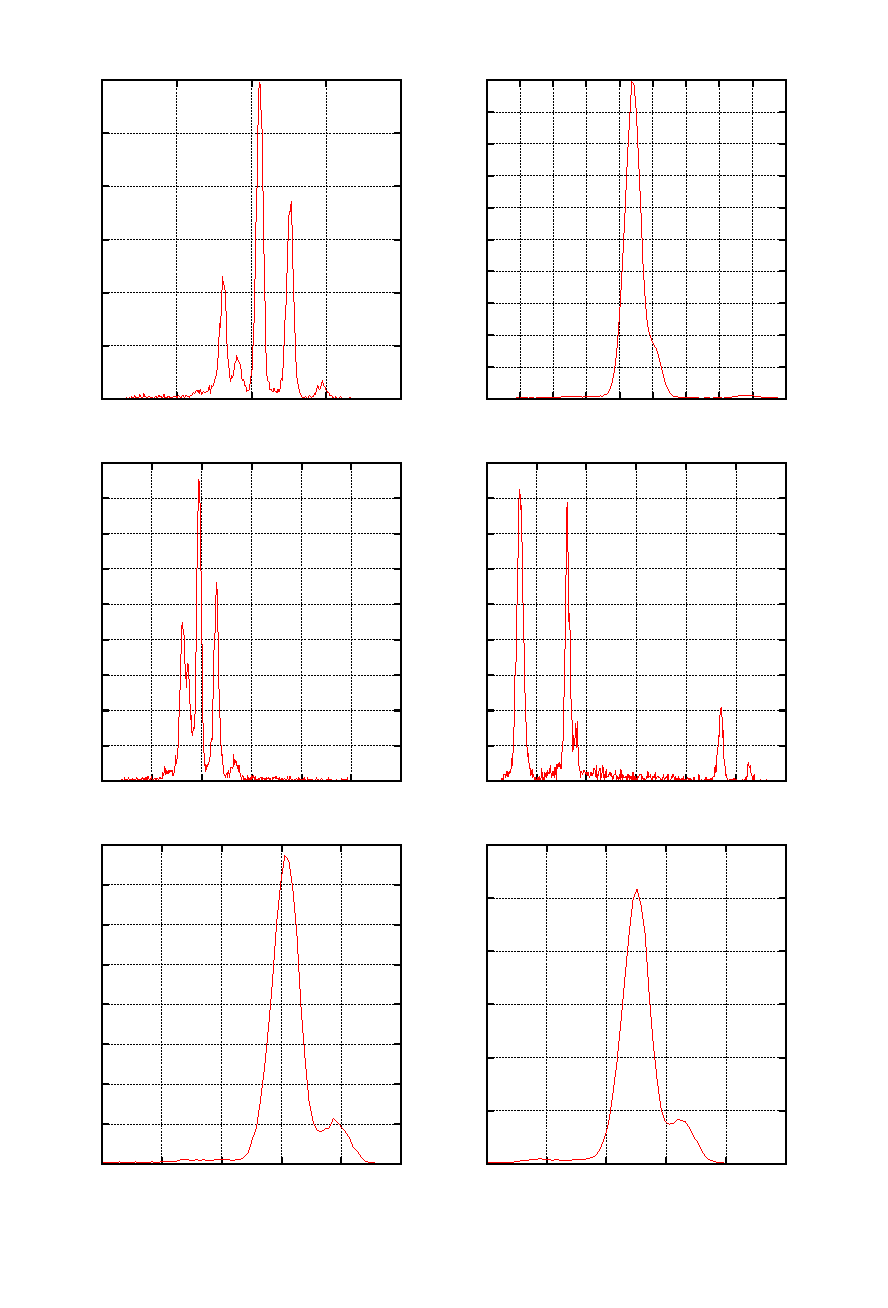
\includegraphics{./plots/referenzspektren1}}%
    \gplfronttext
  \end{picture}%
\endgroup
